\documentclass[a4paper, 11pt, french]{article}

\usepackage[french]{babel}
\usepackage[utf8]{inputenc}
\usepackage[T1]{fontenc}
\usepackage{csquotes}
\usepackage{amsmath,amsfonts,amssymb,mathrsfs}
\usepackage[includeheadfoot, hmargin=2cm, top=0.9cm, bottom = 1.8cm, headsep=2cm]{geometry}
\usepackage{lmodern} %pas pixelisé
\usepackage{engrec,titlesec,lipsum,xcolor}
\usepackage{fancybox}
\usepackage[skins, most]{tcolorbox}
\usepackage[bookmarks={true},bookmarksopen={true}, pdftitle={Cahier des charges}, pdfauthor={Chevalier Romain}, pdfsubject={Caméra domes}, colorlinks=true, linkcolor=black, urlcolor=blue, citecolor=red]{hyperref}
\usepackage{setspace}
\usepackage{stmaryrd}
\usepackage{multicol} 
\usepackage{enumitem}
\usepackage{array,multirow,makecell}
\usepackage{titlesec}
\usepackage{multirow}
\usepackage{hyperref}
\usepackage{listings}
\usepackage{graphicx}
\usepackage{caption}
\usepackage{subcaption}
\usepackage{float}
\usepackage{fancyhdr}
\usepackage[bottom]{footmisc}
\usepackage{footnote}
\usepackage[page,header]{appendix}
\usepackage{titletoc}
\makesavenoteenv{tabular}
\makesavenoteenv{table}

\graphicspath{{Figures/}{Photos/}}

\usepackage{tikz}
\usepackage{pgfplots}
\usetikzlibrary{decorations.pathmorphing, shapes, automata,positioning}



%-----------------------------------------------------------------------------------

\pagestyle{fancy}
\renewcommand{\headrulewidth}{1pt}
\fancyhead[C]{\leftmark} 
%\fancyhead[R]{\includegraphics[scale=0.13]{logoAdeoService.jpg}}
\fancyhead[R]{
\includegraphics[scale=0.1]{Logo_CENTRALE_C.png}}
\newcolumntype{M}{>{\centering\arraybackslash}m{1.75cm}}
\setlength{\headheight}{30.5pt}

%-----------------------------------------------------------------------------------

\frenchbsetup{StandardLists=true}
%\setlength{\parskip}{1em}
\AddThinSpaceBeforeFootnotes
\FrenchFootnotes

%---------------------------------------------------------------

%-----------------------------------------------------------------------------------

\definecolor{vert}{rgb}{0,0.69,0.31}
\definecolor{bleue}{rgb}{0,0.31,0.69} 
\definecolor{violet}{rgb}{0.38,0.18,055} % 97, 45, 140     244, 208, 63
\definecolor{jaune}{rgb}{0.96, 0.85, 0.23}

\definecolor{darkWhite}{rgb}{0.94,0.94,0.94}
\definecolor{vert}{rgb}{0,0.69,0.31}
\definecolor{rose}{rgb}{1,0.08,0.58}% rgb(255,20,147)
\definecolor{rouge}{rgb}{0.78,0.12,0.08}
\definecolor{gris}{rgb}{0.4,0.4,0.4}
\definecolor{marron}{rgb}{0.4,0.2,0}
\definecolor{darkWhite}{rgb}{0.94,0.94,0.94}

%-----------------------------------------------------------------------------------

\title{%
        \Huge Suivi d'un grimpeur par caméra dome \\
        \LARGE Rapport de PDI}

\author{\LARGE CHEVALIER Romain}
\date{\today}

\newcommand{\hsp}{\hspace{20pt}}
\newcommand{\HRule}{\rule{\linewidth}{0.5mm}}

%-----------------------------------------------------------------------------------

\newcounter{obj}
\setcounter{obj}{1}


%-----------------------------------------------------------------------------------


\begin{document}
\pagenumbering{roman}
\begin{titlepage}

    \begin{titlepage}
        \begin{center}
      
          % Upper part of the page. The '~' is needed because \\
          % only works if a paragraph has started.
      
          \textsc{\LARGE École Centrale De Lille}\\[2cm]
      
          \textsc{\huge Projet d'intégration}\\[2cm]
      
          % Title
          \HRule \\[0.4cm]
          { \Huge \bfseries Suivi d'un grimpeur par caméra dome\\[0.4cm] }
      
          \HRule \\[2cm]

          \textsc{\Large Rapport de PDI \\} {\large\today}\\[1.5cm]
          
          \vfill
          % A cahnger pour les caméras installées 
          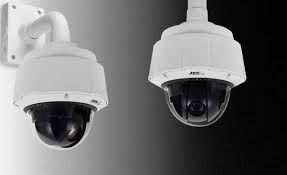
\includegraphics[width=.8\textwidth]{Figures/cameraQ6304.jpg}
          \vfill

          % Author and supervisor
          \begin{minipage}{0.4\textwidth}
            \begin{flushleft} \large
              CHEVALIER Romain\\
            \end{flushleft}
          \end{minipage}
          \begin{minipage}{0.4\textwidth}
            \begin{flushright} \large
              \emph{Tuteur :}  BOURDEAUD'HUY T. \\
            \end{flushright}
          \end{minipage}
      
          \vspace{1cm}
         
        \end{center}
      \end{titlepage}
    
    \normalsize
   
\end{titlepage}

%-----------------------------------------------------------------------------------

\setcounter{secnumdepth}{3}
\setcounter{tocdepth}{3}
\startcontents[sections]

%-----------------------------------------------------------------------------------
\tableofcontents
%\printcontents[sections]{l}{1}{\setcounter{tocdepth}{3}}
%\printcontents[sub]{l}{1}{\setcounter{tocdepth}{2}}
\pagenumbering{arabic}
\newpage

%-------------------------------------------------------------

\section{Contexte}
Afin d'améliorer les services offerts aux utilisateurs de la salle d’escalade \textit{Sac à Pof} situé à  Mons-en-Barœul (59), on envisage de mettre en place un système de suivi automatisé des grimpeurs à l'aide de caméras IP dômes motorisées. Ces caméras permettront de suivre les mouvements des grimpeurs sur les différentes voies en ajustant automatiquement le cadrage et le zoom en fonction de leur position. Le services sera accessible via une application web hébergée sur un serveur local. Cette solution vise à offrir un support d'analyse post-session, afin de permettre aux grimpeur de comprendre leurs forces et faiblesses pour s'améliorer.

Afin de réalisé ce projet, nous sommes en possession de deux caméras IP dômes motorisées de la marque \textit{AXIS} modèle \textit{Q6304-E\footnote{Voir \href{https://www.axis.com/dam/public/11/e4/20/cam\%C3\%A9ra-r\%C3\%A9seau-\%C3\%A0-d\%C3\%B4me-ptz-axis-q6034-e-fr-FR-201515.pdf}{fiche technique} pour plus d'informations}}, d'un routeur, d'une tablette Android et d'un raspberry pi 4.

\subsection{Objectifs}
Les objectifs de ce projet sont multiples et sont résumés dans la liste suivante :
\begin{itemize}
  \item Prendre en main les caméras IP dômes motorisées et les intégrer dans un réseau local.
  \item Développer une interface web permettant de piloter les caméras, l'enregistrement de video et leur visualisation.
  \item Avoir un retour visuel de la caméra en temps réel sur l'interface web.
  \item Développer une méthode de communication entre l'application web et les programmes de contrôle des caméras.
  \item Développer un algorithme de suivi de grimpeur en temps réel.
  \item Développer une méthode permettant d'enregister sur un stockage une vidéo.
  \item Avoir une application modulable permettant de modifier les caméra et les paramètres de détection.
\end{itemize}

\section{Architecture du système}
\subsection{Architecture matérielle}
Le système est composé de plusieurs éléments qui interagissent entre eux, la figure \ref{fig:architecture} montre l'architecture du système. Le système repose sur un \textbf{Raspberry Pi 4}, qui joue un rôle central en assurant la communication entre les différentes composantes. Il est connecté au réseau local via un \textbf{routeur}, qui agit comme un serveur DHCP, attribuant dynamiquement les adresses IP aux appareils du système.

Les \textbf{caméras Dome IP} sont accessibles via HTTP et envoient leur flux vidéo vers le Raspberry Pi lorsqu’elles sont activées. Ces caméras disposent de positions prédéfinies correspondant aux différentes voies d’escalade, mais peuvent également être orientées dynamiquement par l’utilisateur via la \textbf{tablette} fournie ou tout autre appareil connecté au réseau local.

Le Raspberry Pi exécute un serveur d’application web,ce serveur permet :
\begin{itemize}
    \item de piloter les caméras (changement de position, orientation manuelle),
    \item de gérer les enregistrements vidéo,
    \item de stocker dans une base de données les vidéos enregistrées ainsi que les positions des caméras définies par l’utilisateur.
\end{itemize}

L’enregistrement des vidéos est déclenché manuellement depuis l’interface de la tablette et les fichiers sont conservés jusqu’à suppression par l’utilisateur.

L’architecture ainsi mise en place assure une gestion centralisée et accessible du système, tout en permettant un contrôle précis et flexible des caméras et des enregistrements.


\begin{figure}[!ht]
  \centering
  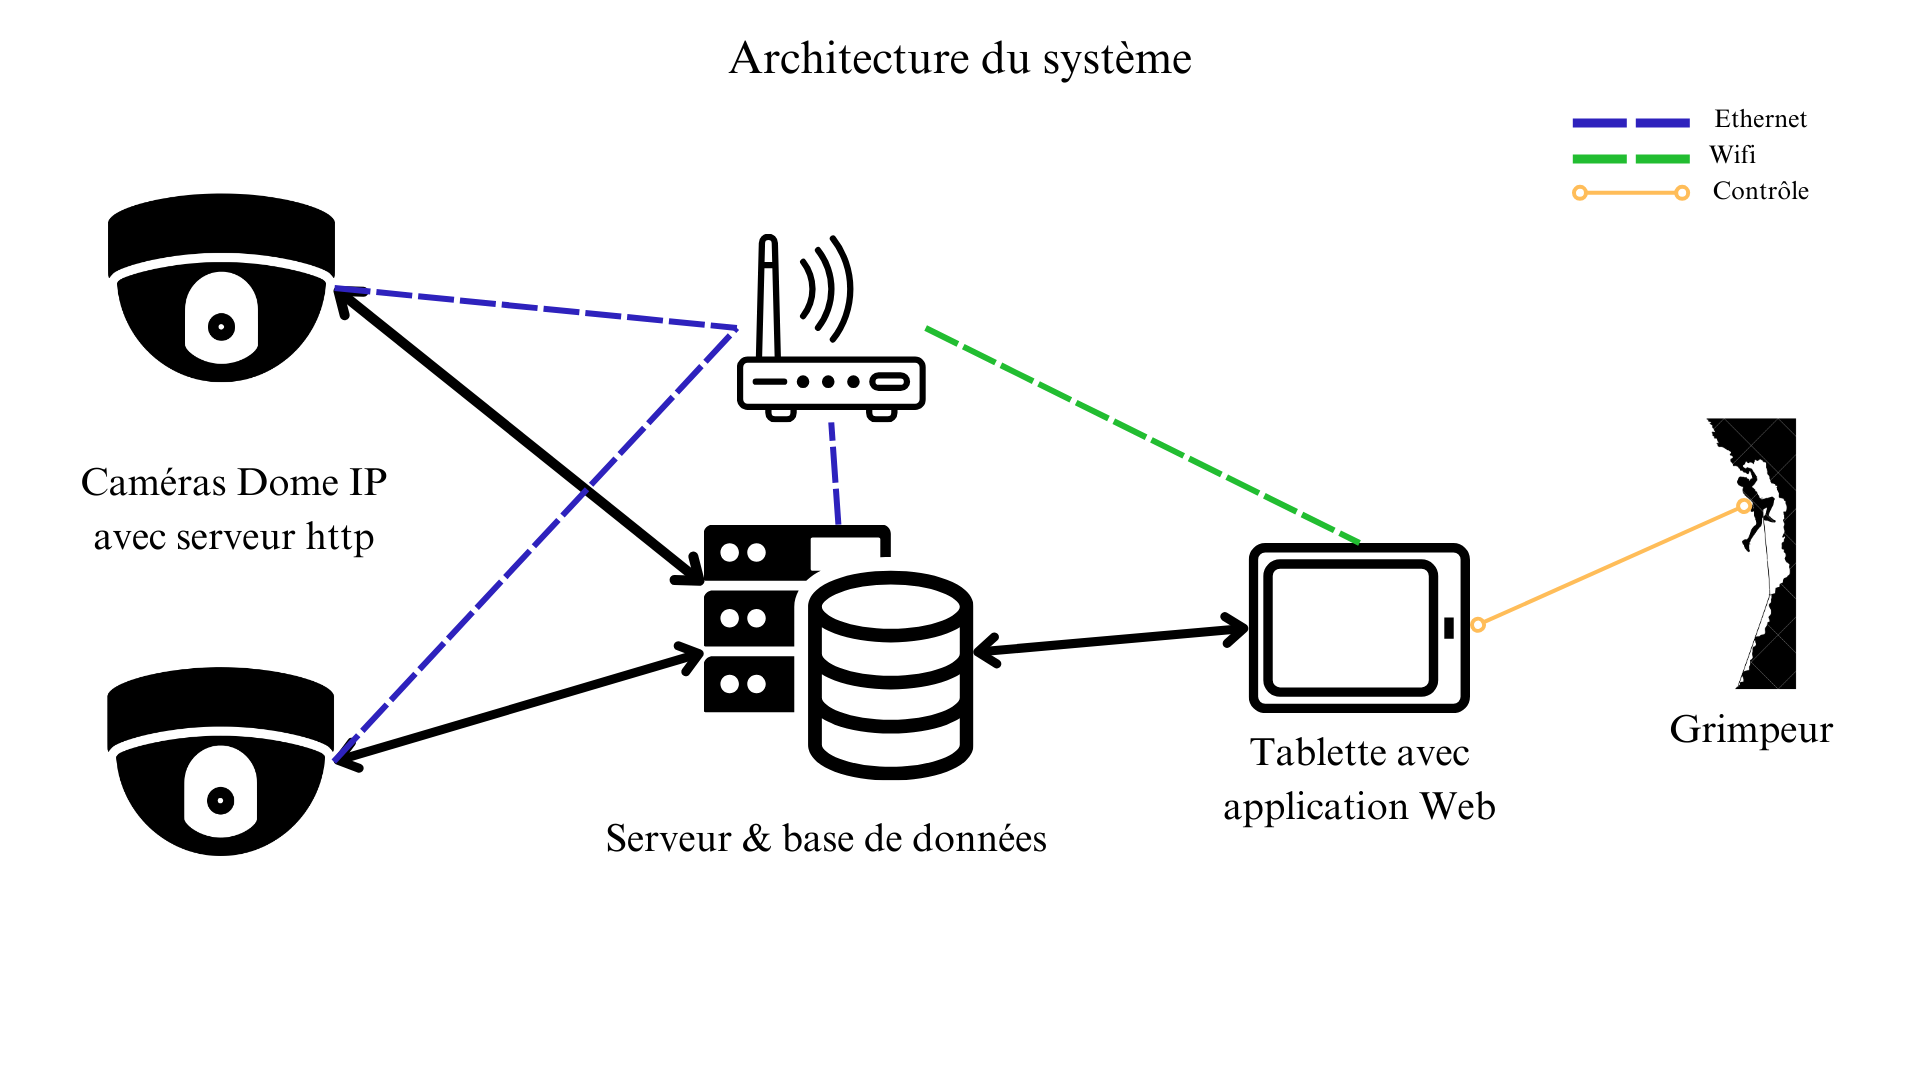
\includegraphics[width=\textwidth]{architectureMaterielle.png}
  \caption{Architecture du système}
  \label{fig:architecture}
\end{figure}

\subsection{Architecture logicielle}
L'architecture logicielle du système est représentée sur la figure \ref{fig:architectureLogicielle}. Le raspberry Pi divise ses tâches en deux parties distinctes : le serveur web et la partie gestion de l'application développée. En fonction des actions effectuées sur la page web, le serveur apache exécuté deux scripts \texttt{cgi} différents, le premier script, nommé \textbf{video.cgi} codé en \texttt{c++}, démarre au chargement de la page permet d'afficher le flux vidéo de la caméra sur la page web en lisant les images brutes dans la mémoire partagée et en les encodant en \texttt{JPEG}. Le second (\textbf{action.cgi} développé en \texttt{c}) permet de transmettre les ordres de déplacement de la caméra ou lancer un enregistrement vidéo via l'écriture de cet ordre dans un segment de mémoire partagé puis de réveillé le programme principal en lui envoyant un signal. 


De l'autre côté, le programme principal (\textbf{main} programmé en \texttt{c}) est en charge de la gestion des caméras, de la détection de mouvement et de l'enregistrement des vidéos. Au démarrage, il crée un processus fils (\textbf{écriture mémoire})qui est en charge de récupérer le flux vidéo du serveur HTTP de la caméra et de le stocker en image brute dans une mémoire partagée. Le programme principal est ensuite en attente d'un signal pour effectuer une action, comme le déplacement de la caméra, l'enregistrement de position ou encore le lancement d'un enregistrement qui va crée un processus fils (\textbf{enregistrement vidéo}) qui encode le flux video en \texttt{MP4} afin de le stocker sur le disque dur et lance la détection du grimpeur pour suivre ces mouvements à l'aide d'un second fils (\textbf{détection}). Ces deux processus récupèrent les images en lisant la mémoire partagée et les traitent pour effectuer leur tâche. Enfin, le programme de détection peut directement agir sur la position de la caméra en lui envoyant une requête HTTP.


\begin{figure}[!ht]
  \centering
  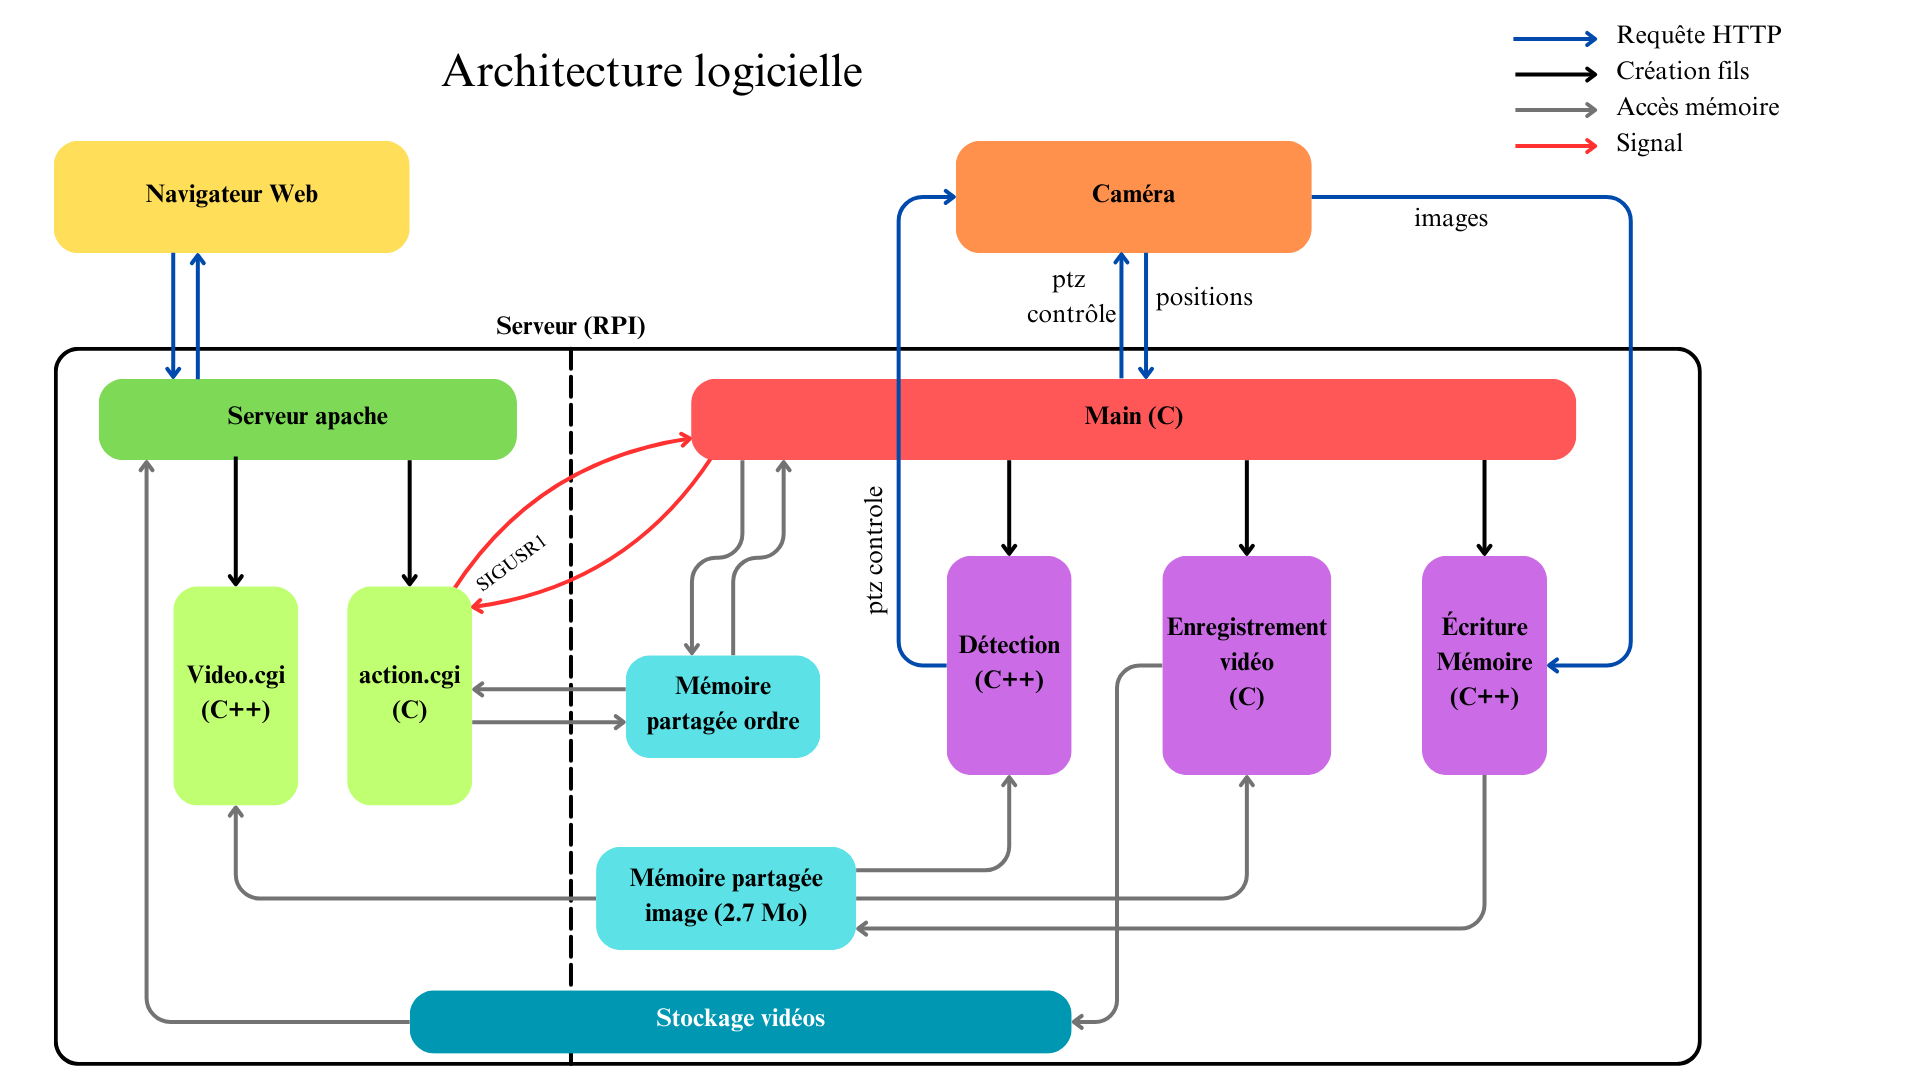
\includegraphics[width=\textwidth]{architectureLogicielle.png}
  \caption{Architecture logicielle}
  \label{fig:architectureLogicielle}
\end{figure}

\section{Développement de l'application}
Dans cette partie, nous allons détailler les différentes étapes de développement de l'application pour chaque brique du système présent dans l'architecture logicielle en figure \ref{fig:architectureLogicielle}.

\subsection{Développement du serveur web}
Le serveur web est composée de deux pages web, la première permet de visualiser le flux vidéo de la caméra, de la piloter et de piloter l'application. La seconde permet de visualiser les vidéos enregistrées et de les télécharger, le code de ces pages est écrit en \texttt{HTML}, \texttt{CSS} et \texttt{JAVASCRIPT} peut-être consulté sur la page \href{https://github.com/Romaiiin91/suiviGrimpeur_PDI/tree/main/server/html}{GitHub}.

\begin{figure}
  \centering
  \begin{subfigure}[b]{0.45\textwidth}
    \includegraphics[width=\textwidth]{pageWeb.png}
    \caption{Index de l'application}
    \label{fig:pageWeb}
  \end{subfigure}
  \begin{subfigure}[b]{0.45\textwidth}
    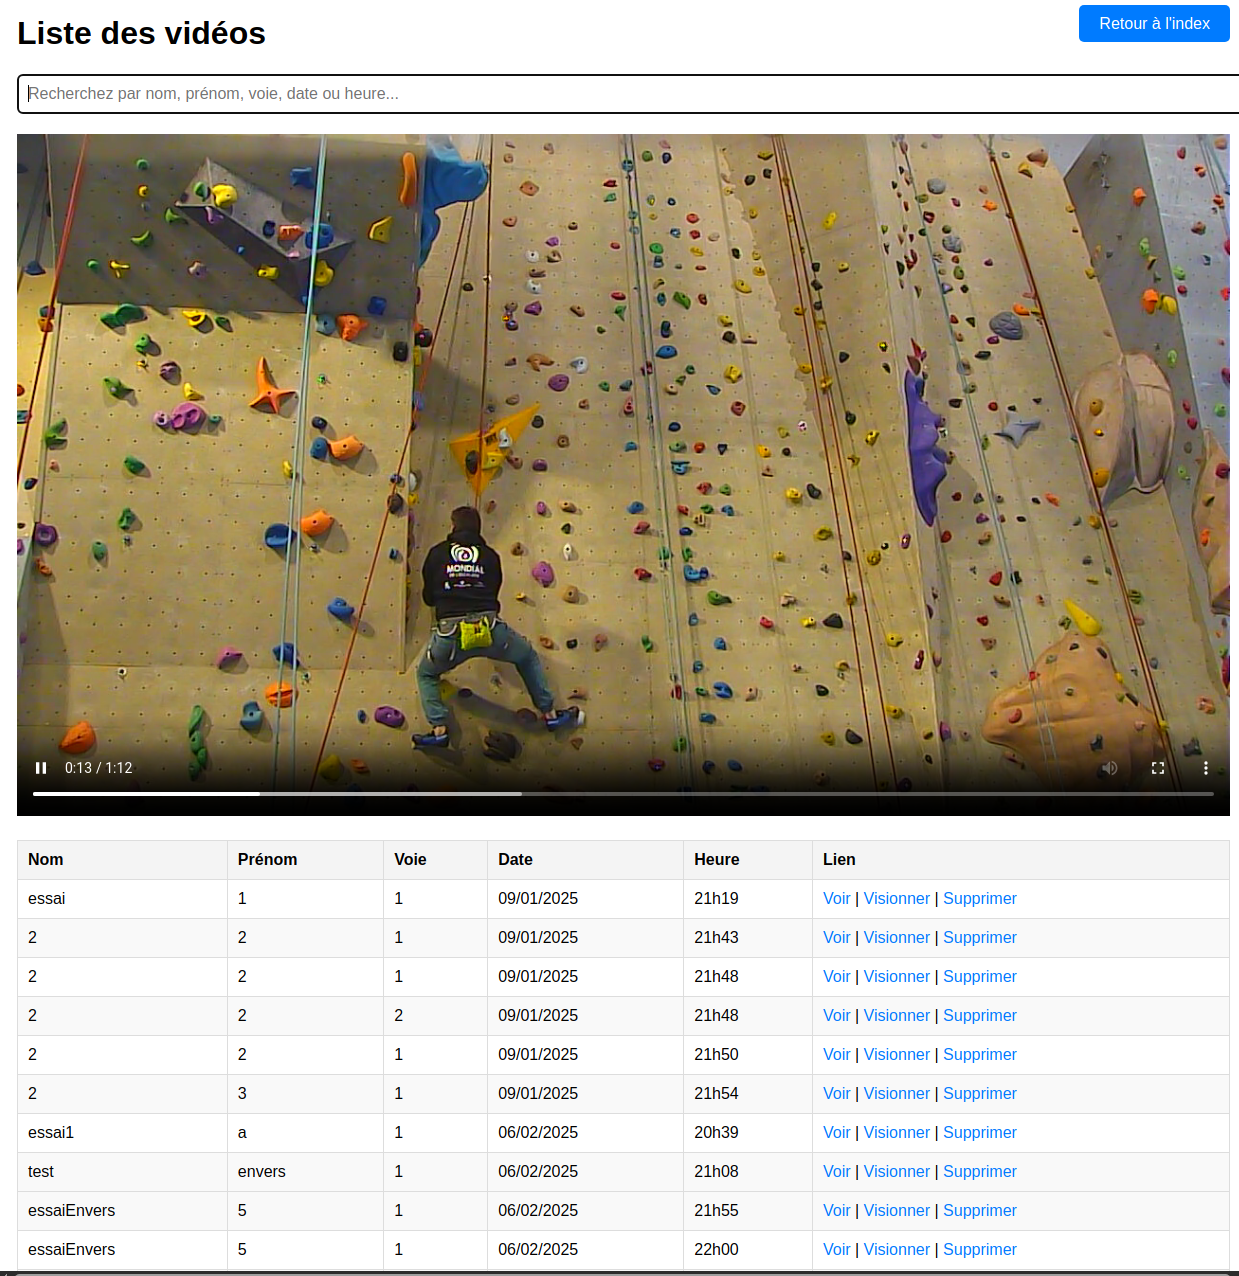
\includegraphics[width=\textwidth]{pageVideo.png}
    \caption{Page web de visualisation des vidéos}
    \label{fig:pageVideo}
  \end{subfigure}
  \caption{Pages web de l'application}
\end{figure}





















%-----------------------------------------------------------
\section{Tests et résultats}

\section{Perspectives d'amélioration}
\begin{itemize}
  \item Amélioration de l'interface Web, avoir une interface plus intuitive et plus ergonomique.
  \item Reformater le code et tout traduire en anglais
  \item Afficher sur l'écran du Raspberry Pi, un meilleur status de l'execution de l'application.
  \item Utiliser les boutons du Raspberry Pi pour relancer l'application.
  \item Ajouter un système de notification pour les erreurs.
  \item Mieux gérer le stockage des vidéos.
  \item Ajouter un système de détection de chute.
\end{itemize}








%-----------------------------------------------------------
% \clearpage
% \newpage


% \section*{Annexes}
% \addcontentsline{toc}{section}{Annexes}

% \appendix

% \startcontents[sections]
% \printcontents[sections]{l}{1}{\setcounter{tocdepth}{2}}


%     \section{Glossaire}
      




\end{document}